\chapter{Turing et Von Neumann}

\section{Un peu d'histoire}
\subsection{La machine de Turing}

En 1936, Alan Turing publie un article de mathématiques, fruit de ses réflexions sur le thème : \og est-il possible de déterminer de manière
mécanique si un énoncé mathématique valide est vrai ou non ? \fg{}.\\
C'est une question cruciale : si sa réponse est \og oui\fg{} cela veut dire qu'il sera peut-être possible de fabriquer une machine qui nous dira si
un énoncé ( par exemple un théorème qu'on aimerait démontrer) est vrai ou non. Plus besoin de démontrer car la machine le fera à notre place !

Turing est amené à proposer un modèle abstrait de machine de calcul que l'on appelle désormais \textit{machine de Turing}.

\begin{figure}[H]
\begin{center}
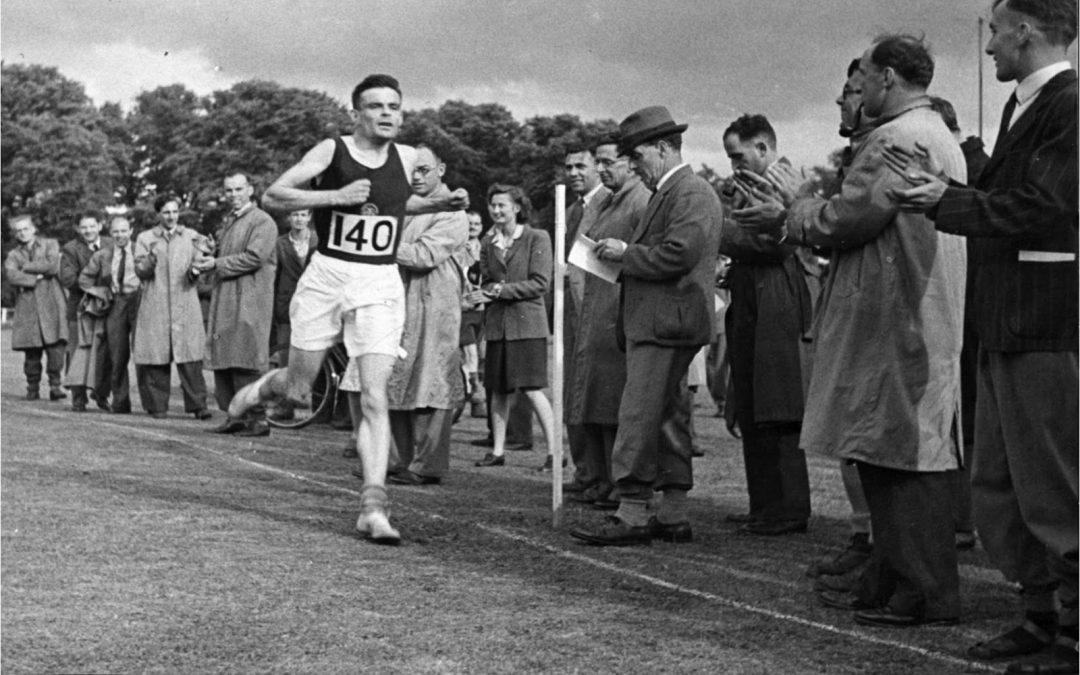
\includegraphics[width=7cm]{img/turing}
\end{center}
\caption*{Alan Turing (1912-1954) était aussi marathonien.}
\end{figure}

Il faut donc imaginer une machine qui peut se déplacer sur un ruban aussi étendu qu'on le désire en avançant ou reculant d'une case à la fois.\\
Définir une machine M c'est se donner
\begin{itemize}
    \item 	un ensemble d'\textit{états} $\mathcal{E}$ dans lesquels la machine M pourra se trouver;
    \item 	un ensemble de \textit{symboles} (un alphabet) $\mathcal{A}$, que la machine peut lire ou écrire sur le ruban;
    \item 	un ensemble de \textit{règles} qui décrivent, selon l'état dans lequel M se trouve et le symbole qu'elle lit, quel symbole elle écrit à
          la place de ce symbole sur le ruban et dans quel sens elle se déplace pour lire le prochain symbole. Cet ensemble de règles peut s'appeler un
          \textit{programme}.
\end{itemize}

\begin{exercice}[]
    Faire l'activité \og Machine de Turing\fg.
\end{exercice}

La machine décrite précédemment ne possède qu'un seul programme. Turing a donc eu l'idée de ce que l'on appelle maintenant une
\textit{Machine de Turing universelle} (MTU).

\begin{figure}[H]
    \begin{center}
        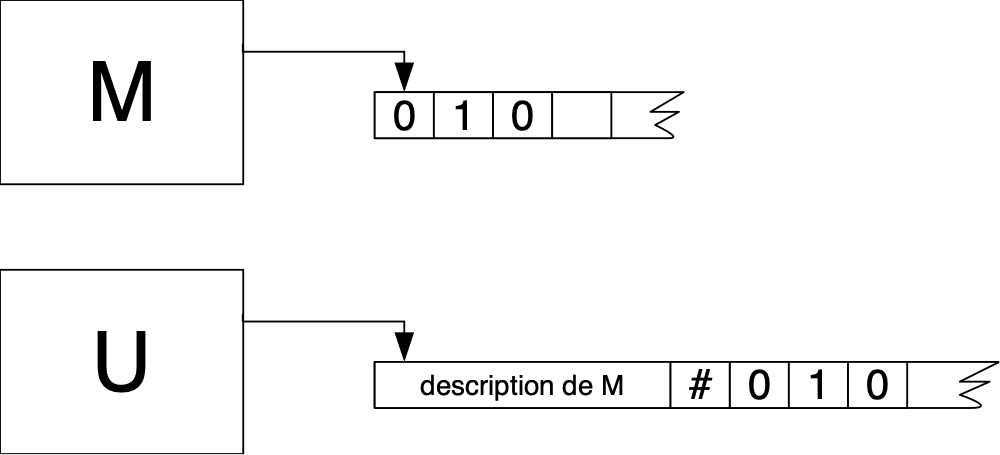
\includegraphics[width=6.5cm]{img/mtu.png}
    \end{center}
    \caption*{Une machine de Truing universelle.}
\end{figure}

Il s'agit d'une machine de Turing U qui est capable de simuler n'importe quelle machine de Turing M,
pourvu qu'on lui fournisse l'ensemble des règles de M et son état de départ. C'est en quelque sorte l'origine de l'ordinateur
programmable, le programme étant les règles de M, et M étant variable.

\subsection{L'ordinateur programmable}

Au milieu des années 40, John Von Neumann et ses collègues ont mis au point une version concrète de l'ordinateur programmable avec une architecture révolutionnaire pour l'époque, qui reste commune à la plupart des ordinateurs actuels et qui porte le nom d'\textit{architecture de Von Neumann}. Celui-ci a expliqué que l'idée de machine de Turing universelle a directement inspiré le projet.

Parmi les premiers ordinateurs figurent l'ENIAC, ordinateur opérationnel à la fin de l'année 1945 et destiné à effectuer des calculs balistiques. C'est une énorme machine, de 90cm d'épaisseur, 2,40m de haut et ... 30,5m de long, le tout pour un poids de 30 tonnes.

\begin{figure}[H]
    \begin{center}
        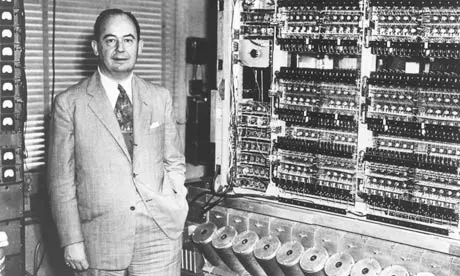
\includegraphics[width=7cm]{img/vonneumann}
    \end{center}
    \caption*{John Von Neumann (1903-1957).}
\end{figure}

Les premières personnes à programmer cet ordinateur sont six femmes, toutes mathématiciennes. L'ordinateur peur réaliser \np{100000} additions par secondes, ou encore 357 multiplications par seconde, ou encore 38 divisions par seconde, le tout avec une capacité mémoire de 20 nombres signés à 10 chiffres en base 10.
\begin{figure}[H]
    \begin{center}
        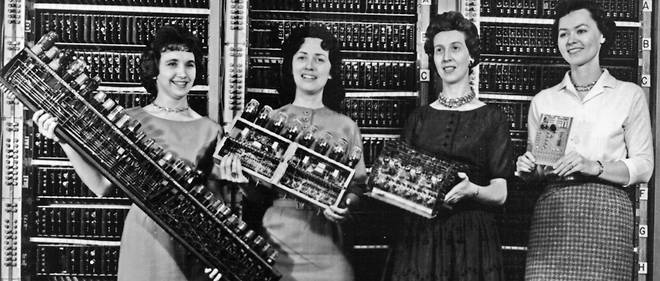
\includegraphics[width=10cm]{img/eniac.jpg}
    \end{center}
    \caption*{Quatre des six programmeuses de l'ENIAC.}
\end{figure}

On peut voir la taille de quelques-uns des \np{17468} tubes à vide qui entraient dans la composition de l'ordinateur. Dès 1947 les transistors ont remplacé les tubes à vides et n'ont cessé d'être miniaturisés. De nos jours les transistors sont directement gravés dans le silicium, leur taille fait quelques nanomètres ($10^{-9}$m) et une carte graphique RTX 2080 en comporte quasiment 20 milliards. La puissance de calcul a beaucoup augmenté puisque le microprocesseur d'un bon PC actuel a une puissance d'environ 150 GFLOPS,  c'est à dire 150 milliards d'opérations sur des nombres en virgule flottante par seconde !

\begin{exercice}[]
    Entre un transistor des années 50 (quelques centimètres) et un transistor actuel, quel est le facteur de réduction de taille ?\\
    Entre l'ENIAC et ses multiplications par seconde et un PC actuel, quel est le facteur d'augmentation de puissance de calcul ?
\end{exercice}

\section{L'architecture de Von Neumann}



Elle décompose l'ordinateur en 4 parties distinctes :
\begin{itemize}
    \item 	l'\textit{unité arithmétique et logique} ou UAL, dont le rôle est d'effectuer des opérations de base;
    \item 	l'\textit{unité de contrôle} et son registre IR, qui est chargée de séquencer les opérations;
    \item 	la \textit{mémoire} qui stocke à la fois les données à utiliser et le programme que l'unité de contrôle va séquencer.
    \item 	les périphériques d'\textit{entrée-sortie} qui permettent de communiquer dans les 2 sens avec l'extérieur.
\end{itemize}

\begin{figure}[H]
    \begin{center}
        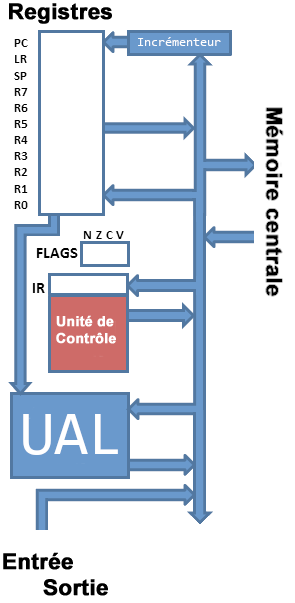
\includegraphics[width=5cm]{img/vn2.png}
    \end{center}
    \caption*{Modèle simplifié de \textit{microprocesseur} (CPU : \textit{Central Processing Unit}).
        Les données transitent par des bus (flèches bleues).}
\end{figure}



Dans le CPU se trouvent des registres :
\begin{itemize}
    \item 	PC (\textit{Program Counter}) qui indique à l'unité de contrôle où aller chercher la prochaine instruction;
    \item 	LR	(\textit{Link Register}) qui contient l'adresse à laquelle le programme doit revenir dans le cas où on aurait appelé un sous-programme (l'équivalent d'une fonction);
    \item 	SP (\textit{Stack Pointer} qui contient l'adresse du sommet de la pile (la pile est un endroit de la mémoire où l'on \og empile\fg{} et \og dépile\fg{} des données, comme une pile d'assiettes);
\end{itemize}
Certaines opérations déclenchent des \og événements\fg{} : quand un résultat est nul, le \textit{flag} (drapeau) Z est mis à un, \textit{et c\ae tera}.

Un processeur donné est capable d'exécuter un nombre d'instructions de base relativement limité. L'ensemble de ces instructions est appelé \textit{langage machine}. Chaque instruction machine est composé d'une ou deux parties :
\begin{itemize}
    \item 	un code opération (appelé \textit{opcode}) qui indique le type de traitement à réaliser ;
    \item 	les données éventuelles sur lesquelles l'opération doit être réalisée.
\end{itemize}

Le fonctionnement d'un CPU est cyclique, la fréquence des cycles étant réglée par une horloge (par exemple un processeur moderne cadencé à 3GHz effectue 3 milliards de cycles par seconde).

\subsection*{Déroulement d'un cycle}

\begin{itemize}
    \item 	le contenu de la RAM pointé par PC est copié dans l'IR de l'unité de contrôle ;
    \item 	l'unité de contrôle décode l'instruction qu'on lui donne et la fait exécuter ;
    \item 	l'exécution provoque l'utilisation des registres, et/ou une lecture ou écriture dans la RAM, éventuellement un accès aux entrées/sorties.
\end{itemize}

Les instructions machine étant \og désespérément austères\fg{} lorsqu'on les écrit en binaire ou en hexadécimal, on les écrit dans un langage compréhensible par les humains. Ce langage s'appelle l'\textit{assembleur}.

\begin{exercice}[]
    Faire l'activité : Simulateur de CPU.
\end{exercice}